\section{Electrons}
\label{sec:ch6_electrons}

\subsection{Reconstruction}
\label{subsec:ch6_electron_reconstruction}

The electron object is reconstructed from an ID track matched to an electromagnetic shower in the calorimeter.
Bremsstrahlung photons emitted in the upstream material can spread the shower energy over several clusters and alter the curvature of the electron track.
Both effects are treated in the reconstruction~\cite{ATLAS2019ElectronPerformance}:
\begin{enumerate}
    \item \textbf{Topo-cluster reconstruction.} Neighbouring cells are grouped into topological clusters according to their signal significance above the expected noise~\cite{ATLAS2017TopoClusters}. Clusters with a substantial electromagnetic energy fraction are used as electron seeds.
    \item \textbf{Track refitting and matching.} Electron-track candidates are refitted with a Gaussian-sum filter, in which a mixture of Gaussian components is used to describe radiative energy losses. The refitted tracks are extrapolated to the second layer of the EM calorimeter and matched to clusters using their differences in $\eta$ and $\phi$. If several tracks match the same cluster, the $\Delta R$ between each extrapolated track position and the cluster centre is used together with the pixel and SCT hits to rank the tracks. The track with the highest rank is selected as the primary electron track. For example, for two matched tracks with $\Delta R=0.02$ and $0.10$ to the cluster centre, the track with the smaller $\Delta R$ is preferred.
    \item \textbf{Supercluster formation.} Nearby clusters are added to the seed to recover energy from bremsstrahlung as shown in Figure~\ref{fig:ch6_electron_supercluster}. Additional clusters sharing the matched electron track can be collected over a wider region in $\phi$.
\end{enumerate}

\begin{figure}[htbp]
    \centering
    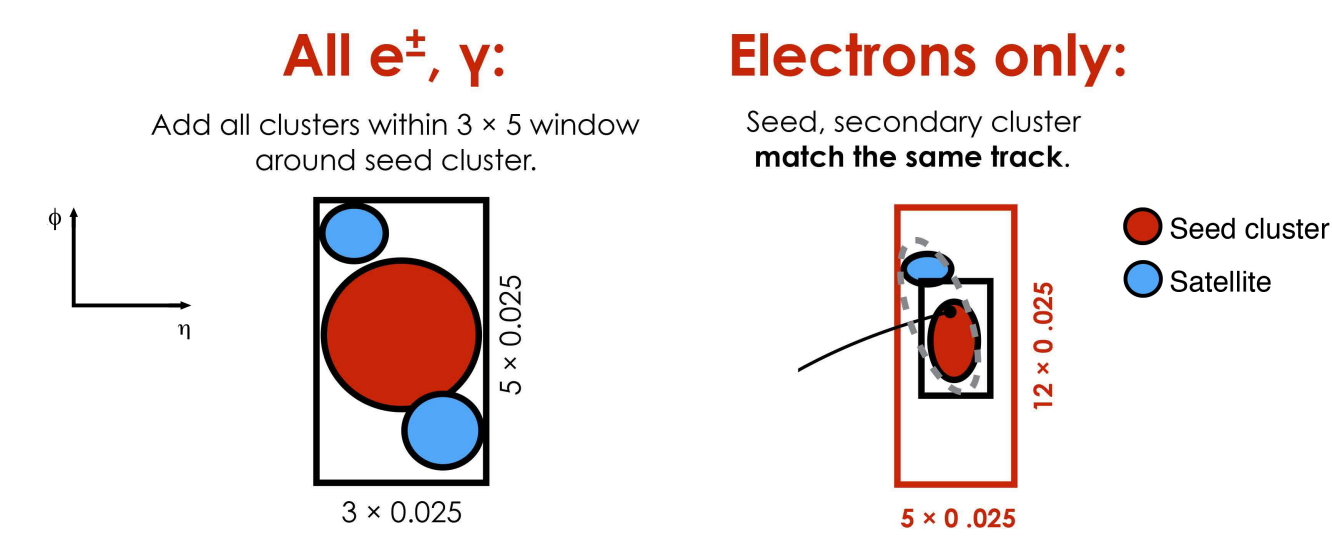
\includegraphics[width=0.75\textwidth]{Figs/CH6/electron_superclusters.png}
    \caption[Cluster association for electron superclusters]{Cluster association for electron superclusters. Seed and additional clusters are shown in red and blue, respectively. Geometrically nearby clusters are collected~\cite{ATLAS2019ElectronPerformance}.}
    \label{fig:ch6_electron_supercluster}
\end{figure}

\subsection{Identification}

Electron candidates are distinguished from hadronic showers and converted photons using a likelihood discriminant~\cite{ATLAS2019ElectronReco}.
Its inputs include the shower shapes in the EM calorimeter, hit variables, and the agreement between the track and calorimeter measurements.
The \texttt{Loose}, \texttt{Medium} and \texttt{Tight} working points are defined with different likelihood-discriminant thresholds and provide increasing background rejection.
The \texttt{Tight} likelihood working point, denoted \texttt{TightLH}, is used for all electron candidates in this analysis.
Its typical prompt-electron identification efficiency is about 80\%, while a representative rejection rate against non-prompt and fake electron candidates in the inclusive QCD background is about 99.5\%~\cite{ATLAS2024ElectronPhotonEfficiencies}.

\subsection{Isolation}

Electrons from hadron decays and jets misidentified as electrons can pass the electron identification requirements.
These electrons are usually accompanied by other particles from the same jet, while prompt electrons typically have smaller nearby track $\pT$ and calorimeter $\et$ sums.
Isolation requirements are therefore used to suppress this background.

Two isolation variables are calculated using tracks and calorimeter clusters within cones around the electron direction:
\begin{itemize}
    \item \textbf{Track isolation} is performed using the $\pT$ sum of tracks in the cone. At high electron $\pT$, other decay products can lie close to the electron due to the boost effect, so the cone radius is reduced.
    \item \textbf{Calorimeter isolation} follows the same principle as track isolation, but uses cluster $\et$ within a fixed cone of $\Delta R=0.2$. The corrected sum estimates the $\et$ from other particles near the electron.
\end{itemize}
In the analysis, baseline electrons are required to pass the \texttt{Loose\_VarRad} isolation working point while signal electrons must additionally satisfy \texttt{HighPtCaloOnly}. They are defined as follows:
\begin{itemize}
    \item \texttt{Loose\_VarRad}: the track and calorimeter isolation sums must be below 15\% and 20\% of the electron $\pT$, respectively.
    \item \texttt{HighPtCaloOnly}: the calorimeter isolation sum is below $\max(0.015\,\pT,3.5~\GeV)$.
\end{itemize}
At high $\et$ ($100<\et<500~\GeV$), the prompt-electron isolation efficiencies are about 99\% for \texttt{Loose\_VarRad} and 90--95\% for \texttt{HighPtCaloOnly}~\cite{ATLAS2024ElectronPhotonEfficiencies}.

\subsection{Calibration}

The calibration consists of an energy calibration, which corrects the measured electron energy, and an efficiency calibration, which corrects the electron selection efficiencies in simulation.
$\zee$ events are used to calibrate the energy and to measure the electron selection efficiencies.
At low electron energies, $J/\psi\rightarrow e^+e^-$ events are used to validate the energy scale and measure the identification efficiency~\cite{ATLASegammaCalibration2015_2016,ATLAS2024ElectronPhotonEfficiencies}.

The energy calibration is applied in the following steps:
\begin{enumerate}
    \item \textbf{Data input corrections.} The relative energy scales of the EM calorimeter layers and the presampler are adjusted using collision data, and the residual energy shifts from pile-up are corrected.
    \item \textbf{MC-based energy calibration.} A BDT-based regression trained on simulated electrons is used to apply an energy correction to data and simulation.
    \item \textbf{Data response uniformity corrections.} Local variations in the energy response are corrected, including those near calorimeter module boundaries and in regions operated at non-nominal high voltage. These corrections improve the uniformity of the measured energy response across the calorimeter.
    \item \textbf{Residual energy scale and resolution calibration.} The remaining energy scale and resolution differences are corrected by comparing the $m_{ee}$ distributions in $\zee$ data and simulation. Electron energies in data are rescaled to match the peak position in simulation, while additional smearing is applied to simulated electron energies to reproduce the width observed in data. The calibration results are further validated with $J/\psi\rightarrow e^+e^-$ events.
\end{enumerate}

For the efficiency calibration, the reconstruction, identification and isolation efficiencies are measured with the tag-and-probe method~\cite{ATLAS2024ElectronPhotonEfficiencies}, in which one electron (the tag) is required to pass strict identification cuts and the other is used as the probe.
After background subtraction, the efficiency is the fraction of probes that pass the selection.
For a selection efficiency $\epsilon$, the scale factor is defined as
\begin{align}
    \mathrm{SF}=\frac{\epsilon_{\mathrm{data}}}{\epsilon_{\mathrm{MC}}}.
    \label{eq:ch6_efficiency_sf}
\end{align}
The scale factors are then applied to simulated event weights for the electron working points used in this analysis to correct the electron selection efficiencies.
